\documentclass[11pt]{beamer}
\mode<presentation>
\let\Tiny=\tiny
\usetheme{CambridgeUS}
\usefonttheme{professionalfonts}
\usepackage[brazil]{babel}
\usepackage[utf8]{inputenc}
\usepackage{amsfonts}
\usepackage{amssymb}
\usepackage{amsmath}
\newtheorem{mydef}{Definição}
\newtheorem{myexample}{Exemplo}

\title{Técnicas e heurísticas para \textit{design} de \textit{interfaces}}
\author{}
\date{}

\begin{document}

    \begin{frame}[plain]
        \titlepage
    \end{frame}

    \begin{frame}
      \frametitle{\textit{Design} de \textit{interfaces}}
      \begin{itemize}
        \item A criação de \textit{interfaces} para \textit{softwares} ganha mais importância após a grande expansão do acesso à \textit{internet}, aos \textit{smartphones} e computadores.
        \item Os \textit{softwares}, antes utilizados apenas por um pequeno grupo de trabalhadores da academia ou de grandes empresas, agora fazem parte da vida da quase totalidade da população dos países mais desenvolvidos.
      \end{itemize}
    \end{frame}

    \begin{frame}
      \frametitle{\textit{Design} de \textit{interfaces}}
      \begin{itemize}
        \item Desenvolver \textit{interfaces} para amplos grupos de pessoas com diferentes culturas, experiências e graus técnicos no uso de computadores torna o desenvolvimento de \textit{software} mais difícil.
        \item Pode-se mitigar este problema através do uso de técnicas e heurísticas já largamente utilizadas na indústria.
      \end{itemize}
    \end{frame}

    \begin{frame}
      \frametitle{Heurística}
      \begin{mydef}
        (Heurística) - uma regra que pode ajudar a resolver um dado problema tomando como base o conhecimento sobre a natureza do problema.
      \end{mydef}
    \end{frame}
    
    \begin{frame}
      \frametitle{Heurísticas de Nielsen}
      \begin{itemize}
        \item Em 1990, dois pesquisadores, Jakob Nielsen e Rolf Molich propuseram 10 heurísticas para auxiliar a criação em \textit{interfaces}.
        \item As heurísticas de Nielsen não são regras extritas, mas parâmetros a serem observados para construção e avaliação de \textit{interfaces}.
      \end{itemize}
    \end{frame}

    \begin{frame}
      \frametitle{Heurísticas de Nielsen}
      São 10 as heurísticas de Nielsen:
      \begin{enumerate}
        \item visibilidade do estado do sistema;
        \item compatibilidade entre o sistema e o mundo real;
        \item controle e liberdade para o usuário;
        \item consistência e padronização;
        \item prevenção de erros;
        \item reconhecimento em vez de memorização;
        \item eficiência e flexibilidade de uso;
        \item estética e design minimalista;
        \item ajude os usuários a reconhecerem, diagnosticarem e recuperarem-se de erros;
        \item ajuda e documentação.
      \end{enumerate}
    \end{frame}
    
    \begin{frame}
      \frametitle{Visibilidade do estado do sistema}
      \begin{itemize}
        \item É quase mandatório que o usuário esteja sempre a par do estado do sistema.
        \item Isso pode ser garantido por elementos de interface pequenos, mas que auxiliam bastante o usuário.
        \item São exemplos de visibilidade do estado do sistema:
          \begin{itemize}
            \item a mudança do símbolo de \textit{play} para o \textit{pause} em aplicativos de músicas;
            \item tempo estimado para o fim de um \textit{download};
            \item barra indicando quanto do espaço de armazenamento foi utilizado;
            \item a seleção da faixa que está tocando.
          \end{itemize}
      \end{itemize}
    \end{frame}

    \begin{frame}
      \frametitle{Visibilidade do estado do sistema}
      Barra de progresso para indicar o quanto de um \textit{download} ou instalação de um \textit{software} foi feito até então.
      \begin{figure}[ht]
        \centering
        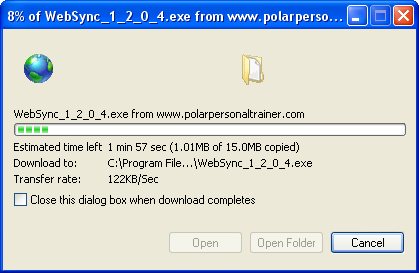
\includegraphics[height=5cm, width=7cm]{figures/download_estimated_time.png}\footnote{Fonte: Flickr/Doug Beckers. Licença: CC BY-SA 2.0}
      \end{figure}
    \end{frame}

    \begin{frame}
      \frametitle{Visibilidade do estado do sistema}
      Ampulheta ou roda para indicar que uma ação está sendo realizada.
      \begin{figure}[ht]
        \centering
        
\includegraphics[height=4cm, width=4cm]{figures/spinning_wheel.png}\footnote{Fonte: FreeSVG. Domínio Público}
      \end{figure}
    \end{frame}
    
    \begin{frame}
      \frametitle{Compatibilidade entre o sistema e o mundo real}
      \begin{itemize}
        \item O sistema deve fornecer uma linguagem familiar ao contexto do usuário.
        \item Por exemplo, se um sistema é voltado para crianças, então a linguagem deve ser compatível com esse público.
        \item Deve-se utilizar ícones que possibilitem ao usuário ter uma noção intuitiva do que um botão faz.
      \end{itemize}
    \end{frame}
    
    \begin{frame}
      \frametitle{Controle e liberdade para o usuário}
      \begin{itemize}
        \item Trata da capacidade do usuário poder desfazer uma ação ou não ser forçado a seguir um único caminho.
        \item Três exemplos clássicos desta heurística:
          \begin{itemize}
            \item a lixeira presente na maioria dos SOs modernos;
            \item a lixeira presente nos sistemas de e-mails;
            \item a função desfazer (Ctrl+z).
          \end{itemize}
      \end{itemize}
    \end{frame}

    \begin{frame}
      \frametitle{Controle e liberdade para o usuário}
      \begin{itemize}
        \item Outro exemplo é poder explorar um \textit{site} de \textit{e-commerce} sem obrigatoriamente ter de fazer \textit{login}.
        \item O \textit{site} da Amazon e um bom exemplo de liberdade para o usuário, pois permite que o usuário remova itens do carrinho durante o \textit{checkout}.
      \end{itemize}
    \end{frame}
    
    \begin{frame}
      \frametitle{Controle e liberdade para o usuário}
      \begin{itemize}
        \item Em alguns casos, será interessante restringir a liberdade do usuário.
        \item Por exemplo, adicionar um \textit{wizard} para instalação e configuração de impressora.
      \end{itemize}
    \end{frame}
    
    \begin{frame}
      \frametitle{Consistência e padronização}
      \begin{itemize}
        \item O sistema deve possuir uma padronização léxica e gráfica.
        \item \textbf{Apenas um ícone ou um termo} devem indicar uma funcionalidade.
        \item Um ícone ou um termo devem indicar \textbf{apenas uma funcionalidade}.
        \item A disposição e o alinhamento de ícones, botões e textos também deve ser consistente.
      \end{itemize}
    \end{frame}

    \begin{frame}
      \frametitle{Prevenção de erros}
      \begin{itemize}
        \item A \textit{interface} deve ser projetada para que o usuário cometa o menor número de erros possíveis.
        \item São exemplos os sistemas que sugerem uma busca com ortografia parecida ou de sinônimos da que foi buscada e a inserção de máscaras, dicas marginais e caixas de confirmação buscam garantir esta característica.
        \begin{figure}[ht]
          \centering
          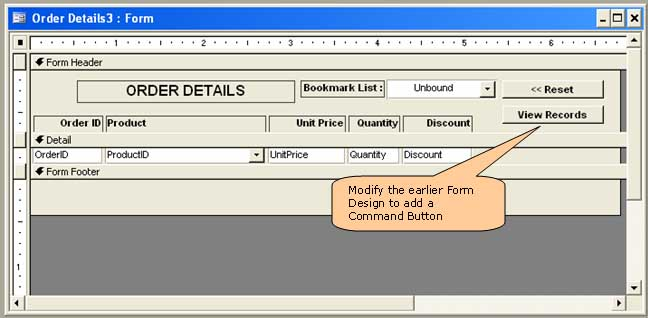
\includegraphics[height=4cm, width=6.5cm]{figures/tips.jpg}\footnote{Fonte: msaccesstips.com. Licença: CC BY-NC-ND 2.5}
        \end{figure}
      \end{itemize}
    \end{frame}
    
    \begin{frame}
      \frametitle{Reconhecimento ao invés de memorização}
      \begin{itemize}
        \item Objetos, ações e opções devem ser visíveis ao usuário.
        \item O usuário não deve ter de lembrar da informação de uma parte do sistema em outra. Este deve estar sempre visível quando necessária.
        \item Sistemas que dependem de códigos são um mau exemplo.
      \end{itemize}
    \end{frame}

    \begin{frame}
      \frametitle{Flexibilidade e eficiência de uso}
      \begin{itemize}
        \item A \textit{interface} além de ser bastante visual para os usuários mais inexperientes, também deve possuir ``aceleradores'' para os usuários mais avançados.
        \item São exemplos desses ``aceleradores'':
          \begin{itemize}
            \item teclas de atalho;
            \item boas opções padrão em formulários;
            \item sistemas de recomendação.
          \end{itemize}
      \end{itemize}
    \end{frame}
    
    \begin{frame}
      \frametitle{Estética e \textit{design} minimalistas}
      \begin{itemize}
        \item Tanto a distribuição das cores quanto das informações não deve atrapalhar o usuário.
        \item Não se deve inserir funcionalidades ou elementos de \textit{interface} que não serão utilizados.
      \end{itemize}
    \end{frame}

    \begin{frame}
      \frametitle{Recuperação de erros}
      \begin{itemize}
        \item As mensagens de erro devem ser claras e de fácil entendimento para o usuário.
      \end{itemize}
    \end{frame}

    \begin{frame}
      \frametitle{Ajuda e documentação}
      \begin{itemize}
        \item É importante que haja uma seção dedicada à ajuda e à documentação.
        \item Muitas vezes o usuário necessitará buscar mais detalhes sobre uma determinada funcionalidade, portanto, é importante que as seções de ajuda e documentação sejam bem arquitetadas e com linguagem simples e direta.
      \end{itemize}
    \end{frame}
    
    \begin{frame}{Referências}
      \begin{itemize}
        \item Dix, Alan \textit{et al.}. Human-Computer Interaction. 3ed. Pearson Education. 2004.
        \item Editora Alea. Nielsen's Heuristics: 10 Usability Principles to Improve UI Design. https://aelaschool.com/en/interactiondesign/10-usability-heuristics-ui-design/. 2022.
      \end{itemize}
    \end{frame}    
\end{document}